% vim: set tw=0:
\documentclass{beamer}
\usepackage{graphicx}
\usepackage{hyperref}
\hypersetup{pdfborder={0 0 0 0}}

% Reasonable themes:
% Antibes Bergen Berkeley Berlin Frankfurt Goettingen Ilmenau Luebeck Malmoe
% Montpellier PaloAlto Rochester Singapore Szeged Warsaw bars boxes
% compatibility default lined plain shadow sidebar split tree
% And these ones include the author's name on every slide:
% Berkeley

% Declare themes.
\mode<presentation>
\usetheme{UWHEP}

% Personal macros.
\newcommand{\email}[1]{{\texttt #1}}
\newcommand{\newframe}[1]{\section{#1}
    \frametitle{\sc{#1}}}
\newcommand{\subframe}[1]{\subsection{#1}
    \frametitle{\sc{#1}}}
\newcommand{\supers}[1]{\ensuremath{^\textrm{#1}}}
\newcommand{\subs}[1]{\ensuremath{_\textrm{#1}}}
\newcommand{\ca}{\ensuremath{\sim}}
\renewcommand{\email}[1]{\href{mailto:#1}{\nolinkurl{#1}}}

% Author information.
\title{T2 Status}
\author[Maier, Mohapatra]{
    Will Maier \and Ajit Mohapatra\\ 
    {\tt wcmaier@hep.wisc.edu}\\
    {\tt ajit@hep.wisc.edu}}
\institute[Wisconsin]{University of Wisconsin - High Energy Physics}
\date{2009.06.09}
\logo{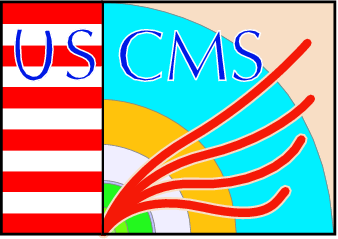
\includegraphics[height=0.6cm]{../../../Graphics/USCMS_logo.png}\hspace{.1cm}
\includegraphics[height=0.75cm]{../../../Graphics/UW_logo.png}}

\begin{document}

\begin{frame}
    \titlepage
\end{frame}

%\section{Overview}
%\begin{frame}
%    \tableofcontents
%\end{frame}

\section{Facilities}
\subsection{Software and Storage}
\begin{frame}
\frametitle{}
\begin{itemize}
	\item Orphaned files filled up dCache
	\begin{itemize}
		\item File removals succeed (and unlink the path in PNFS)\ldots{}
		\item \ldots{}but file remains on pools
		\item PNFS cleaner problem? Debugging with OSG-Storage
		\item When full, many dCache operations fail (breaking SAM, user jobs, etc)
		\item Script removed \ca{}250TB of orphaned data
		\item Orphaned files still accumulating
	\end{itemize}
	\item New dashboard feature for monitoring `popular' datasets by site
	\begin{itemize}
		\item Inspired by external script run at Wisconsin for several months
		\item Helps data managers decide which datasets to remove and whom to contact before removal
		\item Prototype: \url{http://dashb-ssb-devel.cern.ch/dashboard/request.py/listinputcollections}
	\end{itemize}
\end{itemize}
\end{frame}

\subsection{Production and Monitoring}
\begin{frame}
\frametitle{}
\begin{itemize}
	\item (All monitoring suffered during 2009.05.24-28 due to orphaned files)
	\item JobRobot: OK
	\item SAM: OK
	\item RSV: OK
	\item PhEDEx: OK
  \begin{itemize}
		\item LoadTest and MC data transfers in the Debug and Prod instances are doing OK
	\end{itemize}
	\item MC Production:
	\begin{itemize}
		\item Started a new DPG (2.5M) sample this morning
		\item Finishing up the last few Summer08 Alpgen
		\item Using the 2nd Caltech Cluster and the new Omaha cluster
		\begin{itemize}
			\item Brian noticed that CMSSW\_229 was missing on Omaha cluster
			\item Requested Bockjoo to install 229 there
		\end{itemize}
	\end{itemize}
	\item Installed local server running DBS\_206 
	\begin{itemize}
		\item Verified the functionality (registering files) with a test WF in the PA
		\item Will put DBS database in a central MySQL DB server;  DBS server will run on a separate machine
		\item Tested/verified this mode of operation too
	\end{itemize}
\end{itemize}
\end{frame}

\end{document}
